
\paragraph{} Para poder tener una vista mas agradable sobre los diversos episodios del juego, se implemento un visualizador que permite hacer un seguimiento de los movimientos del agente durante un juego. Para poder utilizarlo solo es necesario correr el archivo Main.py de la carpeta rl.visualizer (utiliza la libreria pygame). Para poder elegir que secuencia de movimientos se quiere seguir, basta con modificar el archivo ToVisualize.py seteando la variable MOVEMENTS con alguna de las secuencias que se pueden obtener de los archivos de trace. Ejemplo:

\begin{enumerate}
	\item  Del archivo Dyna-bombR-trace.out se copia la secuencia [3, 3, 3, 3, 1, 4, 0, 2, 5, 8, 3, 1, 1, 6, 2, 4, 3, 1, 1]
	\item  Dentro del archivo ToVisualize.py se escribe MOVEMENTS = [3, 3, 3, 3, 1, 4, 0, 2, 5, 8, 3, 1, 1, 6, 2, 4, 3, 1, 1]
	\item Correr el archivo Main.py
\end{enumerate}


\paragraph{}Una vez que se corre el programa, se debe tener en cuenta las siguientes abreviaciones de teclado:

\begin{itemize}
	\item tecla \textbf{S} o \textbf{SPACE} para empezar o pausar la visualizaci�n
	\item teclas \textbf{UP} o \textbf{DOWN} para modificar la velocidad de los movimientos.
	\item tecla \textbf{F} para pasar a pantalla completa o volver.
	\item tecla \textbf{Q} para salir.
	
	
\end{itemize} 



		\begin{figure}[h!]
			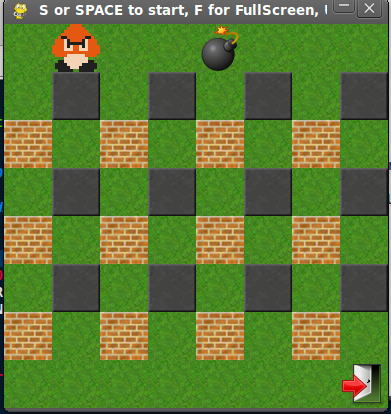
\includegraphics[width=0.3\textwidth]{visualizacion3.png}
			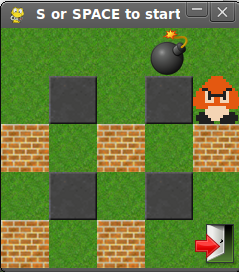
\includegraphics[width=0.3\textwidth]{visualizacion2.png}
			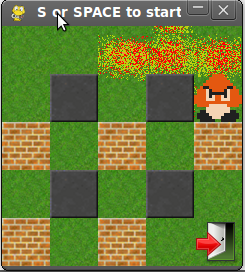
\includegraphics[width=0.3\textwidth]{visualizacion1.png}
			\caption{visualizaci�n}
		\end{figure}
